\documentclass[12pt]{article}
\usepackage[a4paper,top=2.0cm,bottom=1.75cm,left=1.75cm,right=1.75cm,marginparwidth=2.00cm]{geometry}
\usepackage{titlesec}
\usepackage{fancyhdr}
\usepackage{CJKutf8}   
\usepackage{hyperref} 
\usepackage{setspace}
\usepackage{graphicx}
\usepackage{caption}

\usepackage{multirow}
\usepackage{booktabs}
\usepackage{arydshln}
\usepackage{siunitx} 
\usepackage{setspace}

\usepackage[backend=biber]{biblatex}
\addbibresource{references.bib}

\newcommand{\HRule}{\rule{\linewidth}{1mm}} 



\pagestyle{fancy}
\fancyhf{} 
\fancyhead[L]{\textit{Industry-Ready Multilingual TTS Framework} }
\fancyhead[R]{\textit{Masters Research Proposal}}
\fancyfoot[C]{\thepage}


\begin{document}
\begin{CJK*}{UTF8}{gbsn}

\begin{titlepage}
\begin{center}
    \vspace*{2cm}

    % \textit{ Research Proposal \\on}
    研究提案

    \HRule \\[0.3cm]
    { \large \bfseries Industry-Ready Multilingual TTS Framework: Emotion-Aware Voice Synthesis for English, Bengali, and Chinese}\\[0.1cm] 
    \HRule \\[0.3cm]


    \large{ \bfseries \begin{CJK*}{UTF8}{gbsn}硕士研究生申请人\end{CJK*}}
    \vspace*{7cm}
    

    \begin{CJK*}{UTF8}{gbsn}
        \Huge{ \bfseries RAHAMAN NAGIUR(纳吉)}
    \end{CJK*}

    \normalfont{ nagiur@outlook.com \\ +86 184 1906 0056 }
    
\end{center}
\end{titlepage}


\newpage

\onehalfspacing

\section*{引言}

人工智能(AI)的快速发展推动了语音技术领域的显著增长,影响着从娱乐到无障碍的各个行业。对于自然且情感丰富的文本转语音 (TTS) 系统的需求日益增长,这由诸如有声读物、音频剧和互动体验等应用驱动。尽管当前最先进的神经 TTS 模型在英语中表现出色,但在应用于其他语言,特别是资源匮乏的语言(如孟加拉语和中文)时,却面临着巨大的挑战。这些挑战源于语言特定韵律(语调、节奏、重音)和声调变化的复杂性。因此,合成的语音往往缺乏人类声音的情感表达和细微的韵律特征,呈现出机械的品质。\newline

尽管现有的 TTS 模型能够生成可理解的语音,但它们通常难以捕捉人类情感和韵律细微差异的全部范围。这种限制在资源匮乏的语言中尤其严重,因为这些语言的训练数据有限,而且韵律模式也具有独特的特征。此外,控制合成语音中的年龄、性别和情感表达等属性仍然是一个巨大的障碍。这限制了 TTS 的实际应用,使其无法超越基本的转录任务。\newline

本研究旨在开发一个可投入产业应用的多语言 TTS 框架,通过为英语、孟加拉语和中文生成逼真的人声来应对这些限制。该框架将侧重于创建高质量的合成语音,并控制包括年龄、性别和情感表达在内的属性。关键部分是开发能够处理每种语言特定韵律和声调特征的鲁棒模型,特别是孟加拉语和中文的独特特征。这包括解决孟加拉语数据稀缺问题以及改进所有三种语言的韵律建模技术。最终系统将提高合成语音的质量和自然度,从而在更广泛的应用中创建更引人入胜和令人信服的内容。\newline

除了增强讲故事和娱乐功能,该框架还适用于辅助技术、虚拟助手、人工智能驱动的客户服务和教育工具。能够将语音调整为各种情绪状态和说话人特征,将能够在不同的语言和文化背景下提供身临其境的互动体验,从而推动生成语音应用的可能性边界。
\section*{问题陈述}

现有的文本转语音 (TTS) 系统,虽然在自然度方面有所改进,但仍难以生成真正逼真的语音,尤其是在多语言环境和资源匮乏的语言(如孟加拉语和中文)中。这些系统往往缺乏细致的情感表达,无法准确传达各种情绪(快乐、悲伤、愤怒),并且无法根据语音文本的细微差别调整其韵律(语调、节奏、重音)。这种不足在多语言应用和资源匮乏的语言中尤为明显,因为有限的标注数据和捕捉特定文化韵律细微差别的需求极大地增加了任务的复杂性。因此,合成的语音缺乏真实性和人类配音演员的多样化特征,极大地限制了它们在娱乐、教育和无障碍领域的应用。本研究旨在通过开发一个可投入产业应用的多语言 TTS 框架来解决这些限制,该框架能够为英语、孟加拉语和中文合成逼真的人声。该框架将整合先进的情感表达技术,并对语言特定的韵律变化进行建模,从而产生更具表现力和吸引力的数字配音演员。
\section*{Research Objectives}

This research addresses the limitations of current few-shot action recognition by developing and evaluating a novel framework for LLM-guided data augmentation. The core objectives are:

\begin{enumerate}
    \parsep=20pt
    \item \textbf{Develop an LLM-based Action Description Framework:} Leverage LLMs to generate diverse, semantically rich action descriptions, including variations and counterfactual scenarios, evaluated by the relevance and diversity of generated descriptions.
    \item \textbf{Design Augmentation Parameter Mapping:} Implement a method to map LLM descriptions to specific data augmentation parameters (Mixup, CutMix, rotation, etc.), assessed by the realism of augmented samples.
    \item \textbf{Evaluate Augmentation Effectiveness:} Assess the impact of LLM-guided augmentation on few-shot action recognition performance using benchmark datasets (Kinetics, Something-Something, HMDB51) and metrics like N-way K-shot accuracy, comparing against random data augmentation.
    \item \textbf{Compare with State-of-the-Art Methods:} Benchmark the proposed approach against existing few-shot action recognition methods to demonstrate its effectiveness.
    \item \textbf{Analyze Design Choices:} Investigate the impact of different LLM architectures, prompting strategies, and data augmentation techniques to optimize the framework and understand the interplay between LLMs and data augmentation.
\end{enumerate}

\section*{ Research Questions}

The research questions of this study are as follows:
\begin{enumerate}

    \item 
    \item 
    \item 
    \item  
    
\end{enumerate}
\section*{文献综述}

近年来,文本转语音 (TTS) 合成技术取得了显著进展,产生了能够从各种输入(包括短音频提示)生成逼真语音的模型 \cite{shen2018naturalttssynthesisconditioning,ren2022fastspeech2fasthighquality,kim2020glowttsgenerativeflowtexttospeech,kim2021conditionalvariationalautoencoderadversarial} 。这种进步,主要由神经网络架构驱动,对各种应用具有重要意义,从虚拟助手和聊天机器人到音频剧和互动内容创作 \cite{hu2022neuraldubberdubbingvideos,liu2024m3tts} 。然而,当前系统在推广到不同语言时,尤其是在资源匮乏的环境(如孟加拉语和中文)以及传达细致情感时,仍然面临挑战 \cite{chen2024f5ttsfairytalerfakesfluent, eskimez2024e2ttsembarrassinglyeasy}。\newline

自回归 (AR) 模型在 TTS 中是常用方法,已实现令人印象深刻的零样本性能。例如,NaturalSpeech 3 \cite{ju2024naturalspeech3zeroshotspeech} 和 VALL-E 2 \cite{chen2024valle2neuralcodec} 展示了合成各种语音风格的能力。然而,AR 模型通常会面临推理延迟、曝光偏差问题以及需要仔细设计的分词器设计 \cite{song2024ellavstableneuralcodec, du2024valltdecoderonlygenerativetransducer, han2024vallerrobustefficient, peng2024voicecraftzeroshotspeechediting}。这正是非自回归 (NAR) 方法发挥作用的地方,通过并行处理提供了一种有吸引力的替代方案。\newline

扩散模型 \cite{ho2020denoisingdiffusionprobabilisticmodels},特别是那些利用最优传输流匹配 (FM-OT) \cite{kornilov2024optimalflowmatchinglearning} 的模型,在 NAR TTS 系统中已被证明非常有效。这些模型,例如最近的 Voicebox \cite{le2023voiceboxtextguidedmultilingualuniversal} 和 Matcha-TTS \cite{mehta2024matchattsfastttsarchitecture},直接对音频特征的连续空间进行建模,通常无需显式预测音素或持续时间。然而,准确地将输入文本与输出合成语音对齐仍然是 NAR 模型中的一个重大挑战,尤其是在处理这些方法固有的显著长度差异时 \cite{ju2024naturalspeech3zeroshotspeech}。虽然一些模型使用了帧级音素对齐,但最近的研究表明,这种方法对自然度可能不够有效。跳过显式音素级持续时间建模的方法,例如 E2 TTS \cite{eskimez2024e2ttsembarrassinglyeasy} 和 Seed-TTS \cite{anastassiou2024seedttsfamilyhighqualityversatile},通常表现出更自然的韵律。这些模型通常依赖于模型在推理过程中隐式地从整体序列长度推断持续时间。\newline

文献中尤其强调了文本语音对齐的鲁棒性需求,特别是对于多语言 TTS \cite{saeki2024extendingmultilingualspeechsynthesis}。在资源匮乏的语言(如孟加拉语和中文)中普遍存在的数据稀缺问题,需要创新的模型训练方法。数据增强和改进技术在这类情况下有所帮助。DiTTo-TTS \cite{lee2024dittottsefficientscalablezeroshot} 等模型试图通过预训练语言模型整合语义信息。然而,处理对齐和高效合成需求(尤其是在多语言环境中)的最有效方法仍然是研究的重点。本文提出的研究 F5-TTS \cite{chen2024f5ttsfairytalerfakesfluent} 旨在通过一种更简单的方法来构建在现有工作之上,避免显式基于音素的持续时间模型,同时在性能上达到相当甚至可能更好的水平,特别是对于鲁棒性。

总之,TTS 领域正快速发展,正朝着更高效和更灵活的 NAR 模型转变。然而,强大的文本语音对齐以及解决资源匮乏语言的挑战仍然是需要进一步探索的关键领域。本研究旨在通过开发一个强大的多语言 TTS 框架(针对英语、孟加拉语和中文),在合成质量和效率之间取得平衡,特别是考虑到工业级应用需求,来为该领域做出贡献。
\section*{Research Methodology}

The major research findings of this proposal are structured around three phases:  \textbf{(1) Data Preparation}, \textbf{(2) Model Development}, and \textbf{(3) Real-World Application Testing}.


\subsection*{Phase 1: Data Preparation and Feature Engineering}
This phase focuses on the meticulous preparation and structuring of the data required for model training. It involves collecting diverse and high-quality audio corpora for each language, encompassing a range of speakers, ages, and emotions. Essential annotations will specify speaker characteristics, emotions expressed, and the corresponding text. The corpora will be designed to represent various accents, dialects, and speaking styles within each language. Parallel corpora (audio and corresponding scripts) specific to different media (e.g., audiobooks, audio dramas, documentaries) will be collected to capture contextual variations. The data will be preprocessed to address inconsistencies and enhance overall quality through methods like noise reduction, normalization, and segmentation into individual utterances. Automated and manual feature extraction procedures will identify relevant acoustic cues (e.g., pitch, energy, spectral features) and linguistic features (e.g., phoneme duration, pause durations, tonal variations, prosodic contours), crucial for modeling language-specific prosody. The extracted features will be carefully represented in a manner suitable for the model architecture.

\subsection*{Phase 2: Model Development and Training}
In this phase, a novel multilingual TTS framework using a transformer-based architecture will be designed. This framework will incorporate a multimodal encoder to integrate linguistic information, speaker characteristics, and emotional cues. The architecture will include language-specific components to handle the unique prosodic and phonetic characteristics of each language (English, Bengali, and Chinese). The framework will be trained on the prepared corpora using appropriate optimization techniques and loss functions. Rigorous validation will be conducted using held-out portions of the data to evaluate the framework's generalization capabilities. Ongoing evaluation during the training process using relevant metrics (like MOS) will guide the development and refinement of the model. This phase emphasizes iterative model refinement and hyperparameter optimization guided by performance evaluations.

\subsection*{Phase 3: Real-World Application Testing and Evaluation}
This phase evaluates the practical usability of the developed framework. The trained model will be adapted to specific real-world applications (e.g., generating audio for audiobooks, audio dramas, and documentaries). User-friendly interfaces will be designed for potential deployment. A comprehensive evaluation, combining objective metrics (Mean Opinion Score, ASR error rate) and subjective assessments from expert panels (voice actors, linguists, and audio professionals), will be conducted to assess the framework's effectiveness and overall quality in each application context. This evaluation will focus on the naturalness, expressiveness, and cultural appropriateness of the synthesized voices, providing crucial feedback for iterative improvement.

\begin{center}
    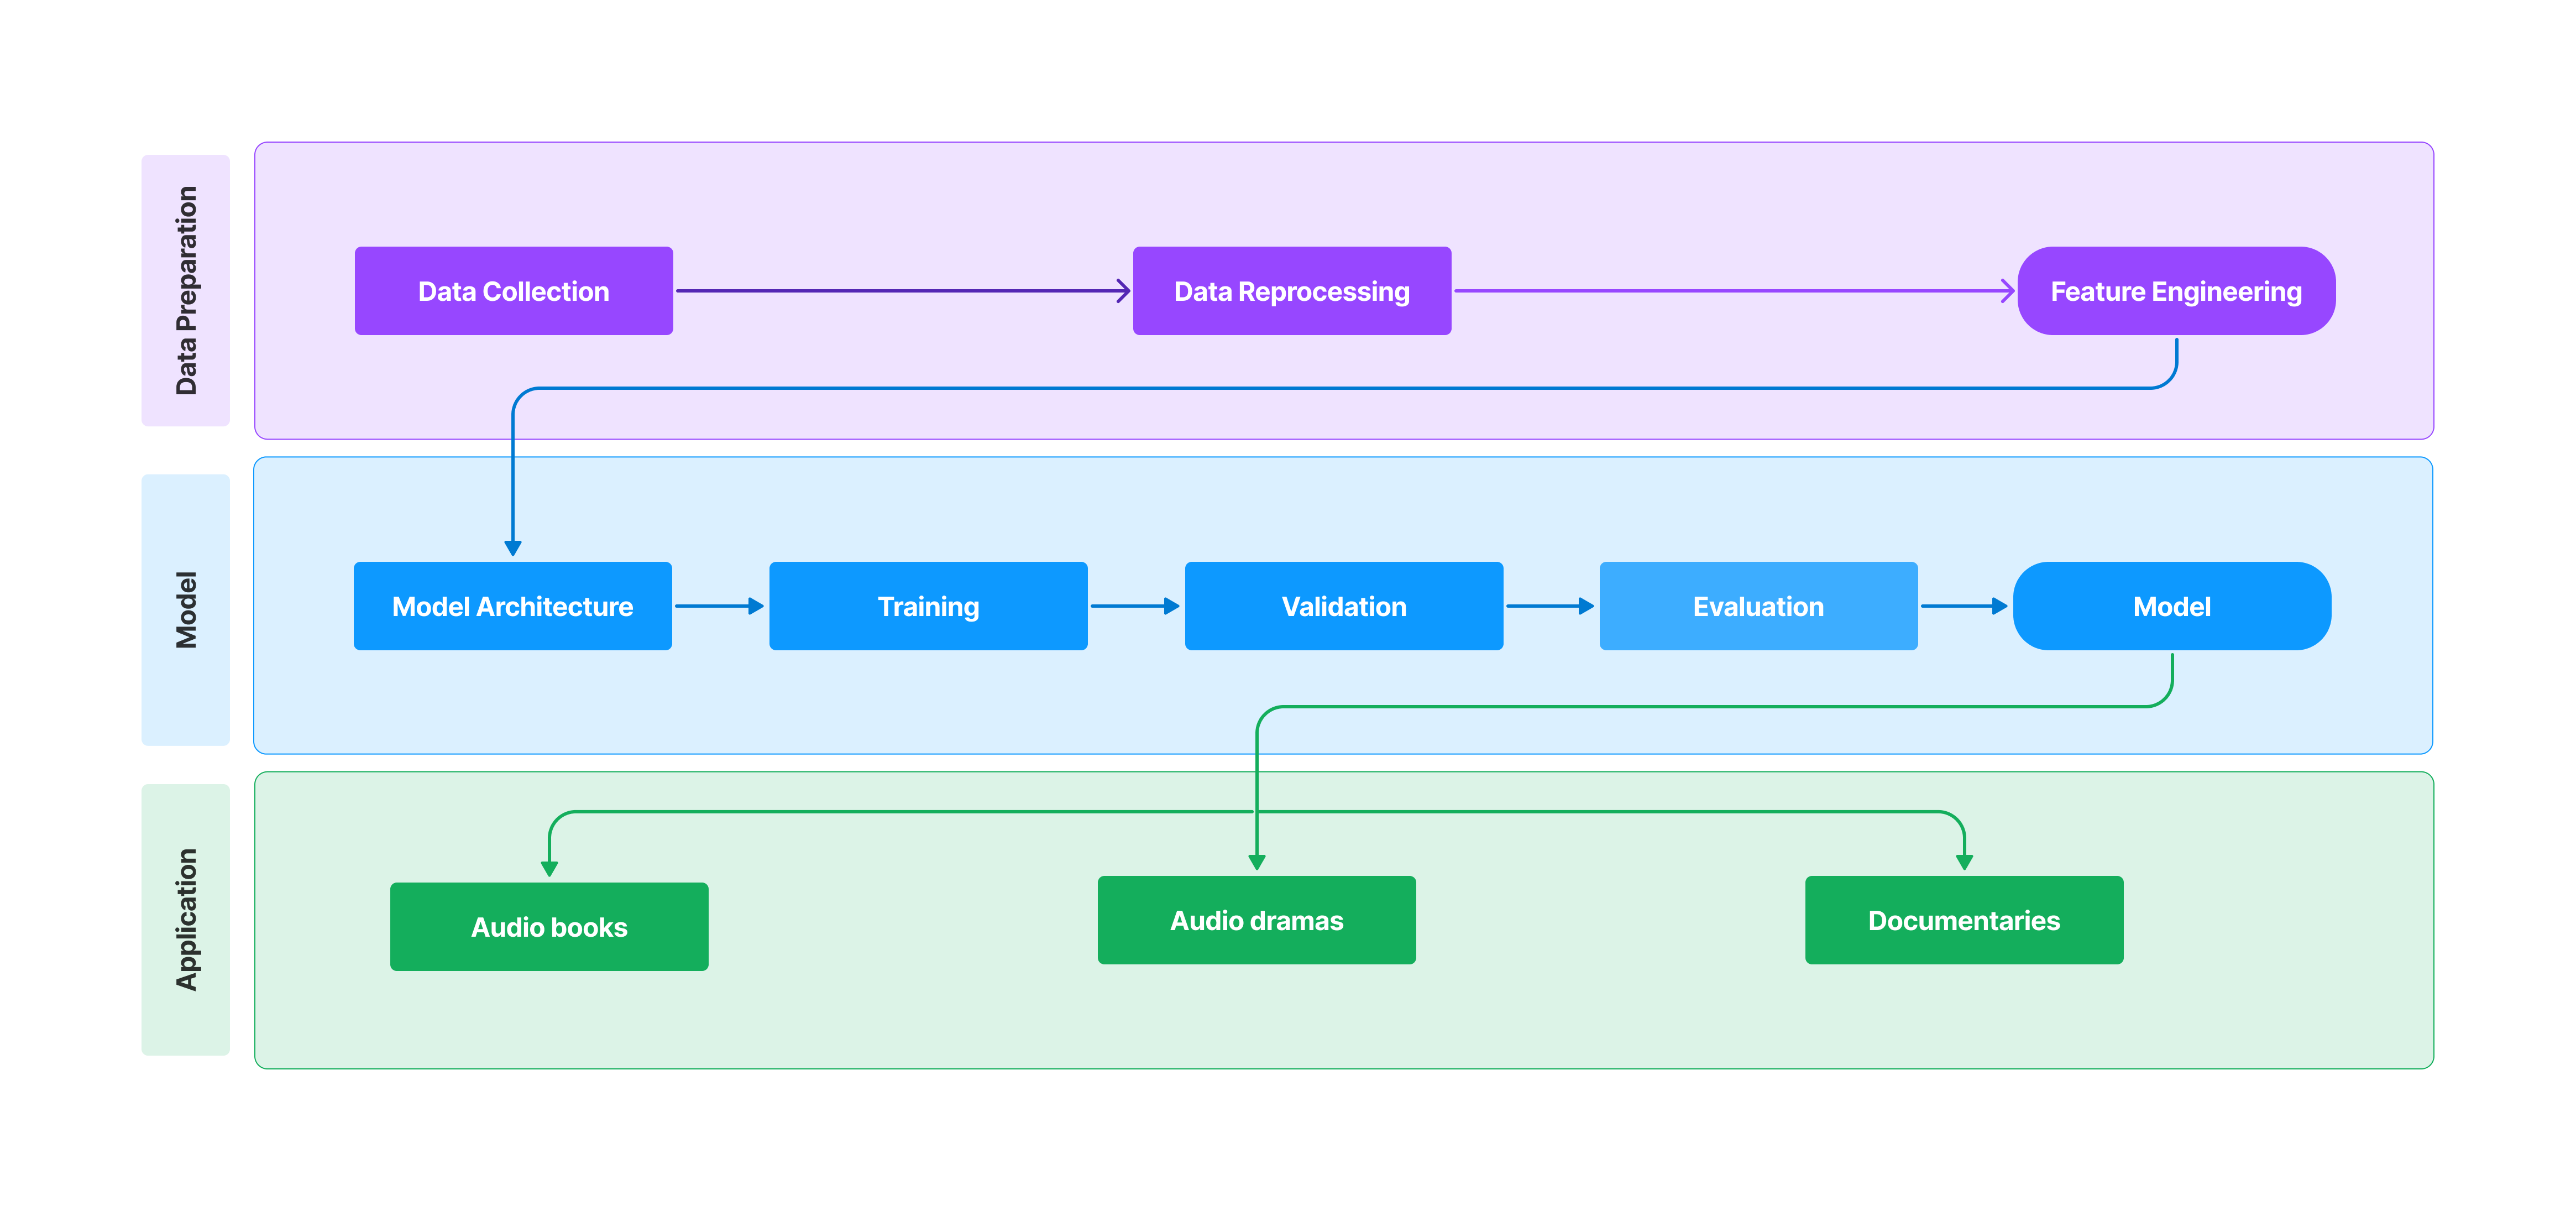
\includegraphics[width=1.0\textwidth]{research-flow.png}
    \captionof{figure}{Research flow}
\end{center}

This methodology employs a phased approach to develop a robust multilingual TTS framework. Data preparation, model development, and real-world testing phases ensure comprehensive evaluation and the framework's suitability for applications like audiobooks and documentaries. The approach prioritizes diverse data, language-specific modeling, and expert evaluation to create a high-quality, practical system.

\section*{预期成果}


\section*{ Timeline}

% The following Gantt chart and table outline the proposed timeline for this research, encompassing key milestones and deliverables. This timeline is subject to adjustments in consultation with my advisor as the research progresses.

% \begin{itemize}
%     \item \textbf{Months 1-2:} Focused Literature Review, culminating in a concise summary of relevant work. Proposal development and defense, resulting in an approved proposal with a scope adjusted for the 12-month timeframe.
%     \item \textbf{Months 3-5:} Fine-tuning a pre-trained LLM for action description generation, potentially focusing on a subset of actions.
%     \item \textbf{Months 4-6:} Development and evaluation of the augmentation parameter mapping model, potentially using a simplified architecture.
%     \item \textbf{Months 6-9:} Experiments on a primary dataset (e.g., HMDB51 or a subset of Something-Something), focusing on key comparisons and analysis.
%     \item \textbf{Months 9-10:} Preparation of a conference paper submission (workshop or shorter paper format).
%     \item \textbf{Months 10-12:} Thesis writing, leading to a completed thesis draft and the thesis defense within month 12.
% \end{itemize}

\begin{table}[h!]
    \centering
    % \caption{Timeline}
    \begin{tabular}{lll}
    % \begin{tabular}{l p{0.4\linewidth} S[table-format=2.0]}


    \toprule
    \textbf{Phase} & \textbf{Description} & \textbf{Duration (months)} \\
    \midrule
    \multirow{2}{*}{\textbf{1. Literature Review}} & Review existing research and & \multirow{2}{*}{2} \\
     & identify research gaps &  \\
     
    
     \midrule
    \multirow{2}{*}{\textbf{2. Data Collection}} & Collect and preprocess datasets & \multirow{2}{*}{3} \\
     & and English speech datasets & \\
    
     \midrule
    \multirow{2}{*}{\textbf{3. Model Development}} & Design and implement the & \multirow{2}{*}{4} \\
     & architecture &  \\

    \midrule
    \multirow{2}{*}{\textbf{4. Training \& Fine-Tuning}} & Train and fine-tune the model on & \multirow{2}{*}{3} \\
     & the collected datasets & \\
    
    \midrule
    \multirow{2}{*}{\textbf{5. Evaluation}} & Conduct subjective and objective & \multirow{2}{*}{2} \\
     & evaluations & \\
    
    \midrule
    \multirow{2}{*}{\textbf{6. Writing \& Reporting}} & Document findings and prepare & \multirow{2}{*}{2} \\
     & research papers or technical & \\
     & reports & \\
    \bottomrule
    \end{tabular}
\end{table}


% \begin{table}[h!]
%     \centering
%     \caption{Timeline}
%     \begin{tabular}{l p{0.4\linewidth} S[table-format=2.0]}
%     \toprule
%     \textbf{Phase} & \textbf{Description} & {Duration (months)} \\
%     \midrule
%     \multirow{2}{*}{Data Preparation} & Review existing research and identify research gaps & 2 \\
%     \midrule
%     \multirow{2}{*}{Data Collection} & Collect and process datasets & 3 \\
%     \midrule
%     \multirow{2}{*}{Model Development} & Design and implement the TTS architecture & 4 \\
%     \midrule
%     \multirow{2}{*}{Training \& Fine-Tuning} & Train and fine-tune the model on the collected datasets & 3 \\
%     \midrule
%     \multirow{2}{*}{Evaluation} & Conduct subjective and objective evaluations & 2 \\
%     \midrule
%     \multirow{2}{*}{Writing \& Reporting} & Document findings and prepare research papers/reports & 2 \\
%     \bottomrule
%     \end{tabular}
% \end{table}   



% References
\printbibliography
\end{CJK*}
\end{document}